\documentclass[12pt,a4paper]{article}
\usepackage[utf8]{inputenc}
\usepackage[spanish]{babel}
\usepackage{graphicx}
\usepackage{listings}
\usepackage{hyperref}
\usepackage{geometry}
\usepackage{tikz}
\usetikzlibrary{shapes.geometric, arrows.meta, positioning}
\geometry{top=2.5cm, bottom=2.5cm, left=2.5cm, right=2.5cm}

\title{\textbf{Trabajo Práctico Integrador -- ARQ-WEB 2026}\\Despliegue, conectividad y verificación experimental de una aplicación web}
\author{Sofia Mereles \and Alba Martinez \and Guillermo Gonzalez}
\date{FP-UNA -- 2026}

\begin{document}

\maketitle

\begin{abstract}
El presente informe documenta la Fase 1 del proyecto integrador de la asignatura Arquitectura Web. En esta etapa se establece la línea base de la infraestructura servidor mediante la configuración de un entorno virtualizado en Ubuntu Server en modo puente (\textit{Bridged}). Se presenta la evaluación comparativa entre dos aplicaciones web de código abierto (BookStack y Ghost), fundamentando la selección de BookStack a través de Registros de Decisiones de Arquitectura (ADR). Finalmente, se valida experimentalmente la conectividad de red, la resolución DNS y los servicios en escucha.
\end{abstract}

\section{Objetivos, Alcance y Criterios de Aceptación}
El objetivo de esta entrega es preparar una infraestructura servidor observable, seleccionar una aplicación web de código abierto apta para su despliegue y verificar las condiciones de red antes del proceso de instalación.

\begin{itemize}
    \item \textbf{Alcance:} Preparación de la VM (2 vCPU, 4 GB RAM, 20 GB Disco), asignación de IP estática/DHCP en capa 3, configuración de OpenSSH, verificación de conectividad bidireccional y definición del esquema de arquitectura lógica de 3 capas.
    \item \textbf{Criterios de Aceptación:} Comunicación ICMP anfitrión-VM sin pérdida de paquetes, acceso saliente a Internet, puerto 22/TCP accesible, cliente DNS operativo y repositorio de versiones inicializado.
\end{itemize}

\section{Selección de la Aplicación Web}

Para la selección del proyecto se evaluaron dos soluciones de código abierto con distintas arquitecturas de software: \textbf{BookStack} (PHP/Laravel) y \textbf{Ghost} (Node.js).

\subsection{Evaluación de Candidatos}

\begin{table}[h!]
\centering
\small
\begin{tabular}{|p{3cm}|p{5.5cm}|p{5.5cm}|}
\hline
\textbf{Criterio} & \textbf{Candidato 1: BookStack} & \textbf{Candidato 2: Ghost} \\ \hline
\textbf{Repositorio} & \url{https://github.com/BookStackApp/BookStack} & \url{https://github.com/TryGhost/Ghost} \\ \hline
\textbf{Licencia} & MIT & MIT \\ \hline
\textbf{Stack Tecnológico} & PHP 8.x / Laravel & Node.js / Express \\ \hline
\textbf{Base de Datos} & MariaDB / MySQL & MySQL 8.0 \\ \hline
\textbf{Servidor Web} & Nginx + PHP-FPM & Nginx + Node.js Process \\ \hline
\textbf{Viabilidad} & Alta (Instalación nativa predecible) & Media (Requerimientos estrictos de Node.js) \\ \hline
\end{tabular}
\caption{Comparativa de candidatos para la selección de la aplicación web.}
\label{tab:candidatos}
\end{table}

\subsection{Aplicación Seleccionada: BookStack}
Tras evaluar la complejidad de despliegue, el mantenimiento y la viabilidad técnica dentro de las cuatro clases del curso, se seleccionó la aplicación \textbf{BookStack}.

\begin{itemize}
    \item \textbf{Repositorio Oficial:} \url{https://github.com/BookStackApp/BookStack}
    \item \textbf{Commit Hash de referencia:} \texttt{cec78b1} (Release v26.05.4)
    \item \textbf{Licencia:} MIT License
    \item \textbf{Lenguaje y Framework:} PHP 8.2+ / Laravel
    \item \textbf{Servidor de Aplicación:} PHP-FPM coordinado con Nginx
    \item \textbf{Base de Datos:} MariaDB 10.11+
    \item \textbf{Puertos previstos:} TCP 80/443 (Nginx Proxy), TCP 3306 (MariaDB interno)
    \item \textbf{Justificación:} Se eligió BookStack debido a su arquitectura clara de 3 capas, su madurez en entornos Linux sobre Nginx/PHP-FPM, la facilidad para inspeccionar logs de sistema y su baja huella de consumo de recursos de CPU y memoria en la VM.
\end{itemize}

\section{Arquitectura del Sistema}

En la Figura \ref{fig:arquitectura_logica} se representa la arquitectura lógica inicial de tres capas diseñada para el despliegue de la aplicación \textbf{BookStack} en la máquina virtual.

\begin{figure}[h!]
\centering
\begin{tikzpicture}[
    node distance=1.8cm and 1.2cm,
    box/.style={draw, rectangle, rounded corners=3pt, align=center, minimum height=1.2cm, minimum width=2.6cm, fill=blue!5, line width=0.8pt},
    net/.style={draw, ellipse, align=center, minimum height=1cm, fill=orange!10, line width=0.8pt},
    arrow/.style={-{Stealth[scale=1.2]}, thick}
]

% Nodos
\node (client) [box, fill=green!10] {\textbf{Cliente HTTP}\\Navegador Web / Host\\\texttt{192.168.100.x}};
\node (net) [net, right=of client] {\textbf{Red LAN}\\Modo Puente\\\textit{Bridged}};
\node (nginx) [box, right=of net, fill=blue!10] {\textbf{Servidor Web}\\Nginx (Proxy)\\Puerto TCP 80/443};
\node (php) [box, below=1.2cm of nginx, fill=purple!10] {\textbf{Aplicación Web}\\PHP-FPM + BookStack\\(Laravel Framework)};
\node (db) [box, left=of php, fill=red!10] {\textbf{Base de Datos}\\MariaDB 10.11+\\Puerto TCP 3306};

% Flechas
\draw [arrow] (client) -- node[above, font=\tiny] {HTTP/HTTPS} (net);
\draw [arrow] (net) -- node[above, font=\tiny] {\texttt{192.168.100.23}} (nginx);
\draw [arrow] (nginx) -- node[right, font=\tiny] {FastCGI / Unix Socket} (php);
\draw [arrow] (php) -- node[above, font=\tiny] {SQL Query} (db);

\end{tikzpicture}
\caption{Diagrama de arquitectura lógica de 3 capas para el despliegue de BookStack.}
\label{fig:arquitectura_logica}
\end{figure}

\subsection{Registro de Decisiones de Arquitectura (ADR)}
A continuación se presentan los Registros de Decisiones de Arquitectura (ADR) que respaldan las selecciones tecnológicas y de infraestructura realizadas para el proyecto.

\subsubsection{ADR-001: Selección de la Aplicación Web de Código Abierto}
\begin{description}
    \item[Estatus:] Aprobado.
    \item[Contexto:] Se requiere desplegar una aplicación web de código abierto en un entorno virtualizado en Ubuntu Server dentro de un marco de cuatro clases, garantizando mantenibilidad, baja huella de recursos y facilidad de observabilidad.
    \item[Decisión:] Se seleccionó \textbf{BookStack} (PHP 8.2+ / Laravel / MariaDB) sobre la alternativa evaluada \textbf{Ghost} (Node.js / Express).
    \item[Consecuencias:] 
    \begin{itemize}
        \item \textit{Positivas:} Arquitectura clásica y predecible de tres capas; excelente compatibilidad con Nginx y PHP-FPM; instalación y resolución de dependencias rápida en Ubuntu Server.
        \item \textit{Negativas / Compromisos:} Requiere la gestión manual de extensiones de PHP y la configuración de permisos en el sistema de archivos local para cargas de medios.
    \end{itemize}
\end{description}

\subsubsection{ADR-002: Modo de Red del Hipervisor (VMware Workstation)}
\begin{description}
    \item[Estatus:] Aprobado.
    \item[Contexto:] La máquina virtual necesita conectividad para la descarga de paquetes desde Internet y accesibilidad directa desde la máquina anfitriona para administración vía SSH y pruebas HTTP.
    \item[Decisión:] Se configuró el adaptador de red virtual en \textbf{Modo Puente (\textit{Bridged})} asignando la interfaz física del host en lugar de red privada NAT.
    \item[Consecuencias:] 
    \begin{itemize}
        \item \textit{Positivas:} La VM obtiene una dirección IP propia e independiente dentro de la red LAN local (\texttt{192.168.100.23/24}), facilitando la prueba de conectividad bidireccional mediante ICMP y SSH sin requerir reglas complejas de reenvío de puertos (\textit{Port Forwarding}).
        \item \textit{Negativas / Compromisos:} Dependencia de la presencia de un servidor DHCP en la red física y mayor exposición del servidor a otros dispositivos de la LAN local.
    \end{itemize}
\end{description}

\subsubsection{ADR-003: Servidor Web y Procesador de Aplicación}
\begin{description}
    \item[Estatus:] Aprobado.
    \item[Contexto:] Se requiere un servidor web para actuar como punto de entrada de peticiones HTTP/HTTPS y servir el contenido dinámico generado por la aplicación PHP/Laravel.
    \item[Decisión:] Se seleccionó \textbf{Nginx} como servidor web / proxy inverso coordinado con \textbf{PHP-FPM} para la ejecución del código PHP.
    \item[Consecuencias:] 
    \begin{itemize}
        \item \textit{Positivas:} Menor consumo de memoria RAM en comparación con Apache HTTPd con \texttt{mod\_php}; alto rendimiento procesando archivos estáticos; separación clara de responsabilidades entre el servidor web y el intérprete de scripts.
        \item \textit{Negativas / Compromisos:} La configuración de reescritura de URLs debe gestionarse centralizadamente en el archivo de bloque de servidor (\textit{server block}) de Nginx, ya que no se soporta el archivo \texttt{.htaccess} de Apache.
    \end{itemize}
\end{description}

\section{Infraestructura y Configuración Base}

\subsection{Repositorio del Proyecto y Control de Versiones}
Como parte de la línea base del proyecto, se creó el repositorio público del equipo y se vinculó con el entorno local de trabajo.

\begin{figure}[h!]
    \centering
    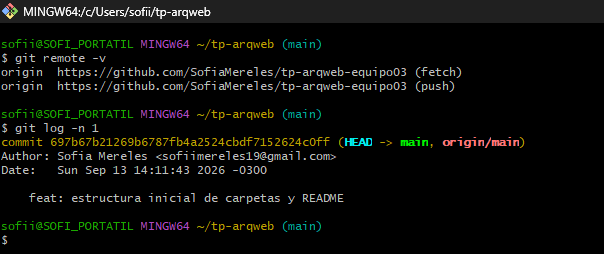
\includegraphics[width=0.85\textwidth]{F1-E1_github_repo.png}
    \caption{F1-E1: Comandos ejecutados en la terminal para la vinculación y confirmación del repositorio local.}
    \label{fig:F1-E1}
\end{figure}

En la Figura \ref{fig:F1-E1} (Evidencia F1-E1), se muestran los comandos ejecutados en la terminal para verificar la dirección remota (\texttt{git remote -v}) y el registro de confirmación inicial (\texttt{git log -n 1}).

\begin{figure}[h!]
    \centering
    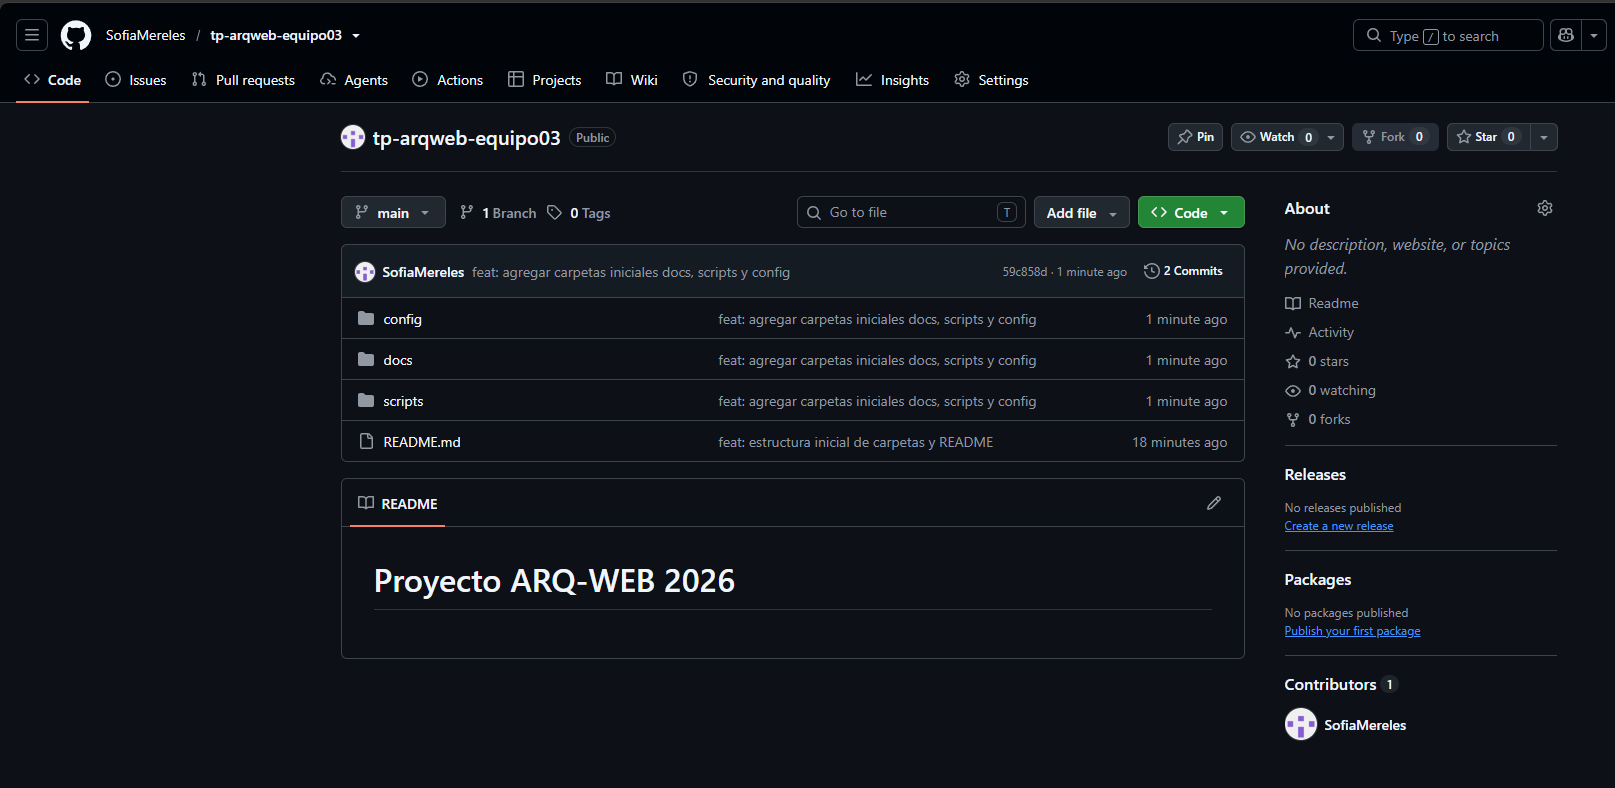
\includegraphics[width=0.85\textwidth]{F1-E2_github_repo.png}
    \caption{F1-E2: Vista web del repositorio público en GitHub con la estructura de directorios.}
    \label{fig:F1-E2}
\end{figure}

Asimismo, en la Figura \ref{fig:F1-E2} (Evidencia F1-E2), se comprueba la sincronización exitosa en la plataforma web de GitHub, reflejando la estructura inicial de directorios del proyecto.

\subsection{Especificaciones de la VM}
\begin{itemize}
    \item \textbf{Sistema Operativo:} Ubuntu Server 24.04 LTS
    \item \textbf{Recursos:} 2 vCPU, 4 GB RAM, 20 GB Disco.
    \item \textbf{Modo de Red:} Adaptador Puente (Bridged).
\end{itemize}

\begin{figure}[h!]
    \centering
    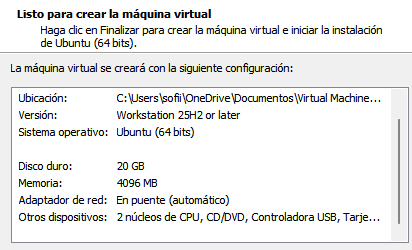
\includegraphics[width=0.85\textwidth]{F1-E3_vmware_hardware.png}
    \caption{F1-E3: Configuración de hardware y red en VMware Workstation (2 vCPU, 4 GB RAM, 20 GB Disco, Adaptador Puente).}
    \label{fig:F1-E3}
\end{figure}

En la Figura \ref{fig:F1-E3} (Evidencia F1-E3), se aprecian las especificaciones asignadas a la máquina virtual dentro del hipervisor VMware Workstation, cumpliendo con los requisitos mínimos de infraestructura definidos para la práctica.

\begin{figure}[h!]
    \centering
    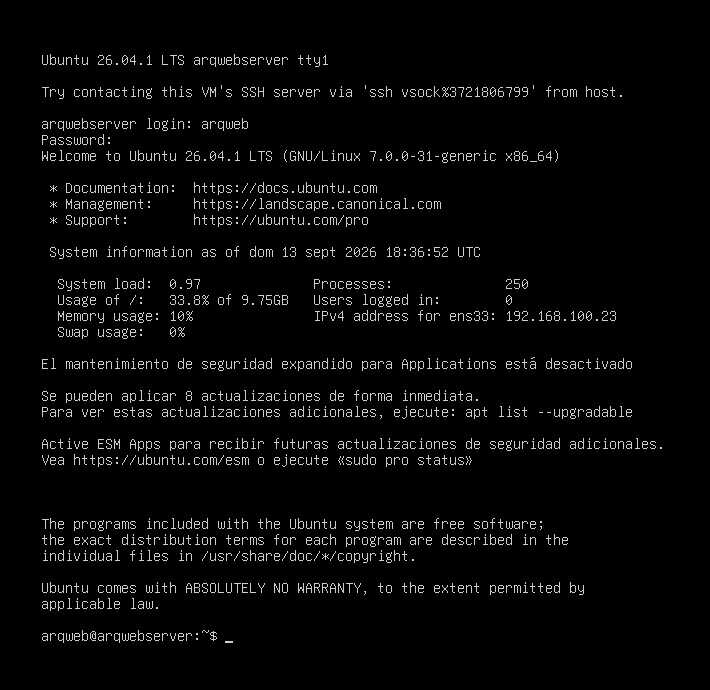
\includegraphics[width=0.85\textwidth]{F1-E4_ubuntu_login.png}
    \caption{F1-E4: Consola de Ubuntu Server operativa con el usuario no-root iniciado.}
    \label{fig:F1-E4}
\end{figure}

Asimismo, en la Figura \ref{fig:F1-E4} (Evidencia F1-E4), se comprueba el inicio de sesión exitoso en el sistema operativo servidor utilizando el usuario no-root configurado con privilegios administrativos mediante sudo.

\subsection{Línea Base de Red y Direccionamiento}
En la máquina virtual se configuró el adaptador de red en modo puente (\textit{Bridged}), lo que le permite obtener una dirección IP dinámica directamente del servidor DHCP de la red local física.

A continuación, se ejecutaron los comandos \texttt{ip addr} e \texttt{ip route} para verificar la interfaz activa y la puerta de enlace predeterminada.

\begin{figure}[h!]
    \centering
    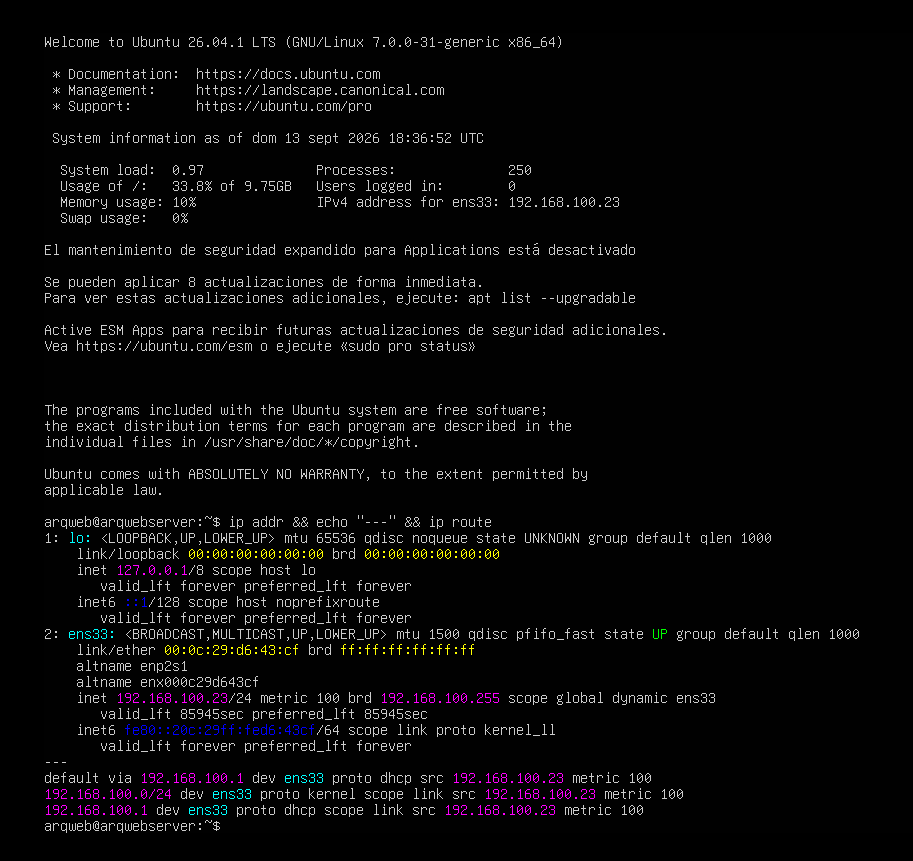
\includegraphics[width=0.85\textwidth]{F1_E5_ip_addr_route.png}
    \caption{F1-E5: Salida del comando \texttt{ip addr} e \texttt{ip route} en Ubuntu Server.}
    \label{fig:F1-E5}
\end{figure}

Como se aprecia en la Figura \ref{fig:F1-E5} (Evidencia F1-E5), la interfaz de red \texttt{ens33} obtuvo exitosamente la dirección IP \texttt{192.168.100.23/24} con la puerta de enlace predeterminada \texttt{192.168.100.1}.

Posteriormente, se realizó la verificación de conectividad bidireccional enviando paquetes ICMP mediante el comando \texttt{ping} entre la máquina anfitriona y la VM, así como también hacia una dirección externa en Internet (\texttt{8.8.8.8}).

\begin{figure}[h!]
    \centering
    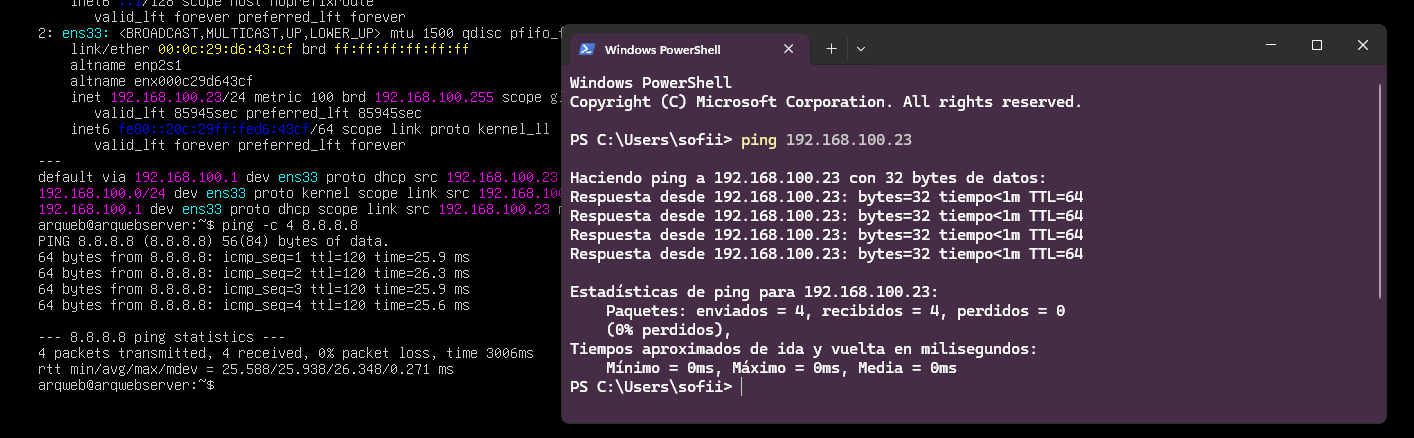
\includegraphics[width=0.85\textwidth]{F1-E6_ping_conectividad.png}
    \caption{F1-E6: Pruebas de conectividad ICMP bidireccional y salida a Internet.}
    \label{fig:F1-E6}
\end{figure}

Como se documenta en la Figura \ref{fig:F1-E6} (Evidencia F1-E6), se confirmó una tasa de pérdida de paquetes del 0\%, validando la comunicación en ambos sentidos y el acceso a la red externa.

Finalmente, se inspeccionó el estado del sistema, los servicios en escucha y la resolución DNS saliente mediante los comandos \texttt{hostnamectl}, \texttt{ss -lntup} y \texttt{curl -I https://ubuntu.com}.

\begin{figure}[h!]
    \centering
    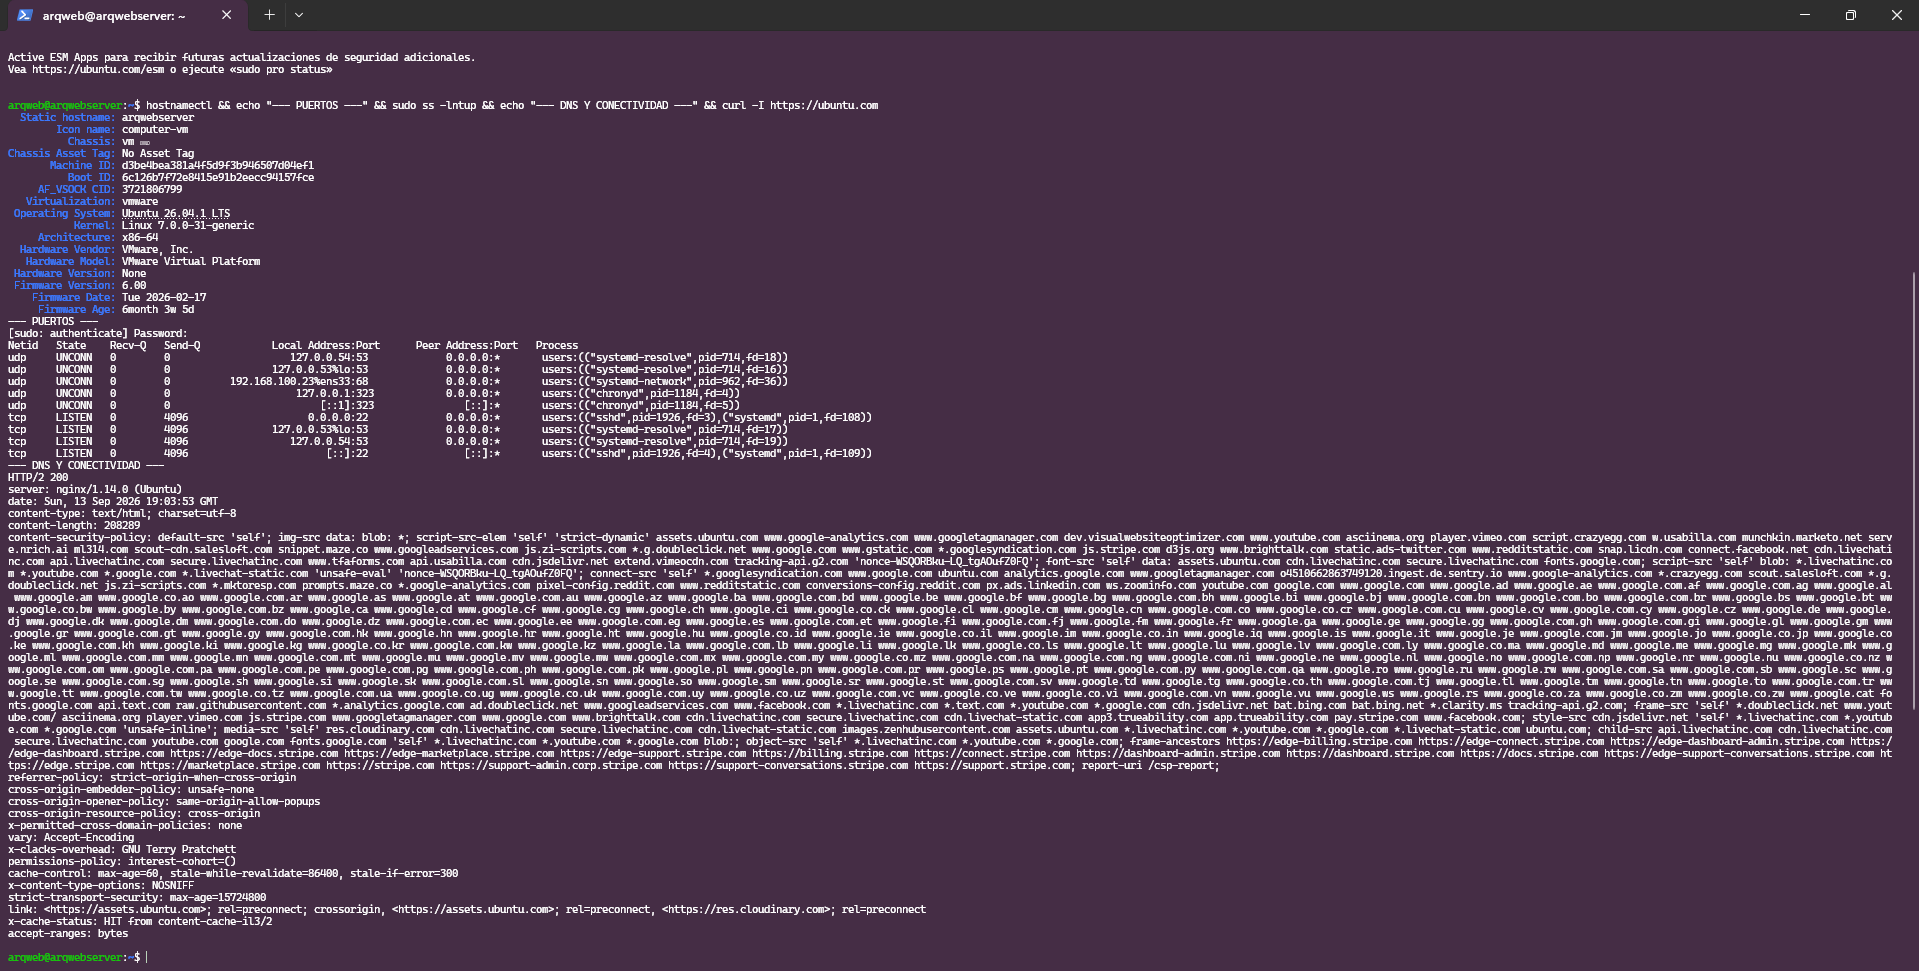
\includegraphics[width=0.85\textwidth]{F1-E7_puertos_dns.png}
    \caption{F1-E7: Verificación del estado del sistema, puertos en escucha (SSH puerto 22) y resolución DNS saliente.}
    \label{fig:F1-E7}
\end{figure}

Como se evidencia en la Figura \ref{fig:F1-E7} (Evidencia F1-E7), se validó que el único servicio expuesto en la red es el servidor OpenSSH en el puerto TCP 22, y se confirmó la correcta resolución de nombres y conectividad web mediante la respuesta HTTP 200 de \texttt{ubuntu.com}.

\section{Matriz de Pruebas y Evidencias}
En la Tabla \ref{tab:matriz_fase1} se presenta el resumen de las pruebas P01, P02 y P03 correspondientes a la Fase 1 del proyecto.

\begin{table}[h!]
\centering
\begin{tabular}{|c|p{3.5cm}|p{6.5cm}|c|}
\hline
\textbf{ID} & \textbf{Dimensión} & \textbf{Prueba y Evidencia} & \textbf{Resultado} \\ \hline
P01 & Direccionamiento & Verificación de IP (\texttt{192.168.100.23/24}) y ruta por defecto (\texttt{192.168.100.1}). Ver Figura \ref{fig:F1-E5} (Evidencia F1-E5). & Exitoso \\ \hline
P02 & Conectividad & Ping bidireccional Anfitrión $\leftrightarrow$ VM y salida externa a Internet (\texttt{8.8.8.8}). Ver Figura \ref{fig:F1-E6} (Evidencia F1-E6). & Exitoso \\ \hline
P03 & Servicios y DNS & Verificación de puertos en escucha (\texttt{ss -lntup}) y resolución DNS saliente (\texttt{curl -I}). Ver Figura \ref{fig:F1-E7} (Evidencia F1-E7). & Exitoso \\ \hline
\end{tabular}
\caption{Matriz de pruebas - Fase 1}
\label{tab:matriz_fase1}
\end{table}

\end{document}